\documentclass{article}
\usepackage[utf8]{inputenc}
\usepackage{geometry}
 \geometry{
 a4paper,
 total={170mm,257mm},
 left=20mm,
 top=20mm,
 }
 \usepackage{graphicx}
 \usepackage{titling}
 \usepackage{amsmath}
 \title{Computer Networks: Assignment 1
}
\author{Priyadarshini Radhakrishnan (2021CS50614), Kartik Meena (2021CS50618)}
\date{August 2023}
 
 \usepackage{fancyhdr}
\fancypagestyle{plain}{%  the preset of fancyhdr 
    \fancyhf{} % clear all header and footer fields
    \fancyhead[L]{Computer Networks}
    \fancyhead[R]{\theauthor}
}
\makeatletter
\def\@maketitle{%
  \newpage
  \null
  \vskip 1em%
  \begin{center}%
  \let \footnote \thanks
    {\LARGE \@title \par}%
    \vskip 1em%
    %{\large \@date}%
  \end{center}%
  \par
  \vskip 1em}
\makeatother

\usepackage{lipsum}  
\usepackage{cmbright}

\begin{document}

\maketitle

\noindent\begin{tabular}{@{}ll}
    Students & \theauthor\\
\end{tabular}

\section*{Network Analysis}
\begin{itemize}
    \item a) Traceroute from mobile hotspot to www.iitd.ac.in via wifi .

    \begin{itemize}
        \item 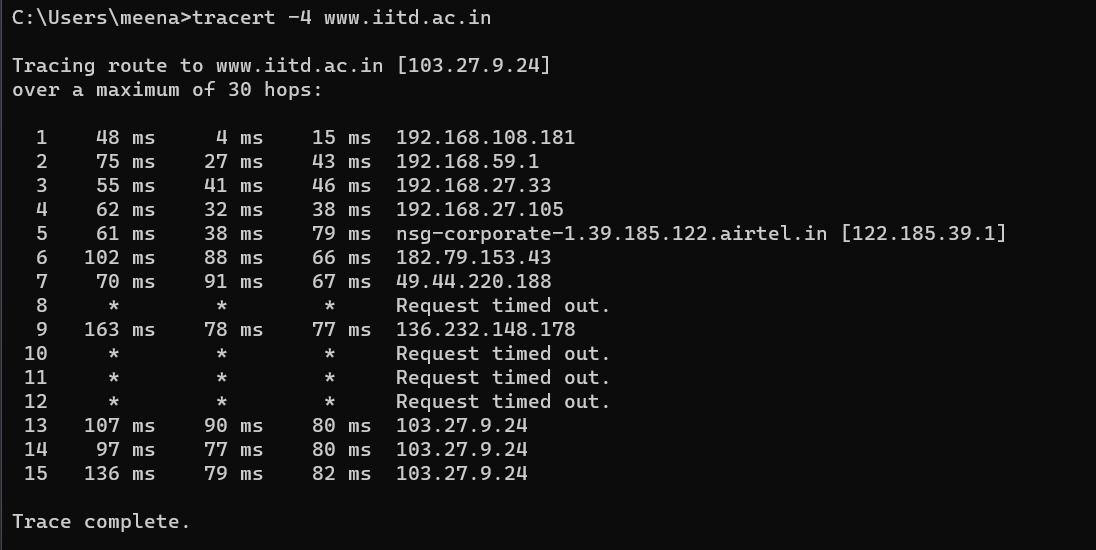
\includegraphics[width=15cm, height=10cm]{Kartik.jpeg}
        \vspace{3mm}
        \item 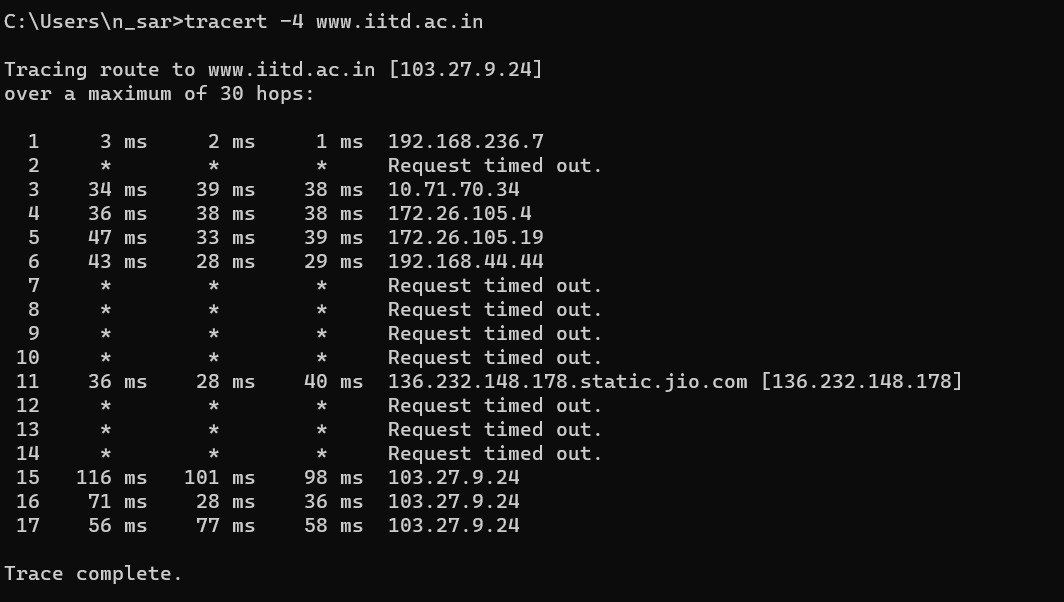
\includegraphics[width=15cm, height=10cm]{WhatsApp Image 2023-08-08 at 6.03.23 PM.jpeg}
    \end{itemize}

    \item b) Curious things noted during the traceroute

    \begin{itemize}
        \item Initially for both the partners client's default IP  was IPv6 address.
        \item Traceroute by default send three packets in every hop.
        \item We can use the command tracert with option -4 to force the traceroute to give all the addresses in IPv4 on windows.
        \item As the laptop was connected to a cellular network hotspot (Airtel 4G Network), its IP address was also present in the hops during the traceroute. This means my packet is also going through the router of Airtel Network. 
        \item Private IP addresses like 192.168.108.181, 192.168.59.1, 198.168.27.33 , 192.168.44.44 ,172.26.105.4, 172.26.105.19  were noted during the traceroute. 
        \item Also, some routers along the path did not seem to reply to the traceroute requests, as the request sent to them was timed out because Time To Live for the packet got expired.
    \end{itemize} 

    \item c) The maximum size of the packets we were able to send using ping is between 0-35300 bytes for www.iitd.ac.in. The link layers determine the maximum permitted size of the packets.
    
\end{itemize}

\section*{Traceroute Using Nping}
\begin{itemize}
    \item \textbf{Choice of Tool}: The tool used is \textbf{nping}. It is configured to send a single echo request and to utilize the TTL value provided by the user.
    \item \textbf{Design Decision}: We chose to send only one packet in the nping command instead of three packets as in traceroute because nping doesn't give individual Round Trip Time.
    \item \textbf{TTL Expiry Handling}: 
        \begin{itemize}
            \item When TTL is expired in transit, the packet is discarded by a router along the path.
            \item Upon TTL expiry, the IP address of the router where the packet is dropped and the round trip time is displayed.
        \end{itemize}
    \item \textbf{Handling Missing Echo Replies}:
        \begin{itemize}
            \item In some cases, the routers might not send an Echo Reply, as the time limit would have exceeded so, "Request timed out" would be displayed.
        \end{itemize}
    \item \textbf{Successful Packet Reach}:
        \begin{itemize}
            \item When the Echo Request packet reaches the destination router and an Echo Reply is received, the traceroute functionality is completed.
            \item Upon successful completion, the output displays the IP addresses of all transit routers, their corresponding RTT values, and a final "Trace Complete" message.
        \end{itemize}
\end{itemize}

\section*{Internet architecture}
\begin{itemize}
    \item \textbf{AS Number for the IP addressess} 
    \begin{center}
\begin{tabular}{|c|c|c|}
    \hline
     AS  & AS Number & IP address  \\
    \hline
    UTAH & 17055 &  155.98.186.21 \\
    \hline
   UCT & 36982 & 137.158.159.192\\
    \hline
    Indian Institute of Technology & 132780  & 103.27.9.24 \\
    \hline 
    Google  &   15169   & 142.250.207.196 \\ 
    \hline
    Facebook & 32934   & 157.240.16.35 \\  
    \hline
    \end{tabular}
\end{center}
    \begin{itemize}
        \item In the  traceroute to www.utah.edu from New York some Autonomous System like west-net-west, INTERNET2-RESEARCH-EDU, NKN-CORE-NW NKN Core Network, are encountered.
        \item In the traceroute to www.uct.ac.za the last known router is TENET-1, ZA(154.114.124.1).
        \item In the traceroute to www.iitd.ac.in from mobile hotspot there are some AS like Reliance Jio Infocomm Limited . IN, BBIL-AP BHARTI Airtel Ltd., IN. 
    \end{itemize}
\end{itemize}
\begin{itemize}
    \item  \textbf{A) Table for the Number of Hopes from Different Sources to the Destination} \\
    \begin{itemize}
    \item Traceroute Source is Equinix New York(NY9) IP address of the source  216.218.252.22 \\ 
    \begin{center}
\begin{tabular}{|c|c|c|}
    \hline
     Destination & Number of Hopes & IP address  \\
    \hline
    www.utha.edu & 15 &  155.98.186.21 \\
    \hline
    www.uct.ac.za & 30 & 137.158.159.192\\
    \hline
    www.iitd.ac.in & 17 & 103.27.9.24 \\
    \hline 
    www.google.com  &   11   & 142.250.207.196 \\ 
    \hline
    www.facebook.com &  8  & 157.240.16.35 \\  
    \hline
    \end{tabular}
\end{center}

   \item Traceroute Source is Equinix Osaka (OS1) IP address of the  source (216.218.252.58), Japan 
   \begin{center}
\begin{tabular}{|c|c|c|}
    \hline
     Destination & Number of Hopes & IP address   \\
    \hline
    www.utha.edu & 16 &   155.98.186.21 \\
    \hline
    www.uct.ac.za & 30 &  137.158.159.192  \\
    \hline
    www.iitd.ac.in & 18 & 103.27.9.24 \\
    \hline 
    www.google.com  &   10  & 142.250.207.196  \\ 
    \hline
    www.facebook.com &  10  & 157.240.16.35 \\  
    \hline
\end{tabular} 
\end{center}
\item Traceroute form my Mobile Network via Wifi \\
        \begin{center}
\begin{tabular}{|c|c|c|}
    \hline
     Destination & Number of Hopes & IP address \\
    \hline
    www.utha.edu & 29 &   155.98.186.21 \\
    \hline
    www.uct.ac.za & 30 &  137.158.159.192 \\
    \hline
    www.iitd.ac.in & 17 & 103.27.9.24 \\
    \hline 
    www.google.com  &   9  & 142.250.195.4  \\ 
    \hline
    www.facebook.com &  9  & 157.240.198.35\\  
    \hline
\end{tabular} 
\end{center}
\begin{itemize}
    \item Special Note for the traceroute of www.uct.ac.za \\
 In this case, the destination did not reply, and traceroute kept incrementing the TTL, the last known router is  154.114.124.1. for all the traceroutes from different sources.
\end{itemize}
\item \textbf{Some Key points observed during the traceroute.}
    \begin{itemize}
        \item \textbf{Effect of Geographical distance of the source from the destination on Hops}: If the traceroute sources and destinations are geographically close, it might generally result in fewer hops. This is because there are likely to be fewer network nodes and routers in between, as there will be less number of routers, gateway, and subnets to pass. However, other factors such as network coverage, traffic, and routing policies can also influence the number of hops. For example, the University of Utah is closer to New York in comparison to Osaka Japan, so traceroute from New York took fewer hops. 
        \item Globally dispersed networks and data centres are present in Google and Facebook. Across many traceroute providers, Google and Facebook display a significant consistency in the number of hops(usually fewer hops). This is because of dedicated pathways, good network protocol policies and optimized routing used by their provider, and these features helps them to establish a big network.
    \end{itemize}          
    
\end{itemize}
\item  \textbf{B) Latencies between the traceroute sources and the web servers} \\
  \textbf{Equinix New York(NY9) IP address of the source  216.218.252.22}
    \begin{center}
\begin{tabular}{|c|c|}
    \hline
     Destination & Range of Latenices(RTT) \\
    \hline
    www.utha.edu & 51.330ms - 58.733ms  \\
    \hline
    www.uct.ac.za &  no packet received \\
    \hline
    www.iitd.ac.in & 221.899ms -  233.809ms  \\
    \hline  
    www.google.com  &  64.457ms - 72.382ms \\ 
    \hline
    www.facebook.com & 78.332ms - 81.868ms \\  
    \hline
    \end{tabular}
\end{center}
\textbf{ Source is Equinix Osaka (OS1) IP address of the source (216.218.252.58)}
    \begin{center}
\begin{tabular}{|c|c|}
    \hline
     Destination & Range of Latenices(RTT) \\
    \hline
    www.utha.edu & 111.609ms - 113.331ms \\
    \hline
    www.uct.ac.za & no packet received \\
    \hline
    www.iitd.ac.in & 256.293ms - 256.563ms  \\
    \hline  
    www.google.com  & 112.806ms - 113.006ms \\ 
    \hline
    www.facebook.com & 140.041ms - 142.211ms \\  
    \hline
    \end{tabular}
\end{center}
\textbf{Source is cellular mobile network via wifi  }
    \begin{center}
\begin{tabular}{|c|c|}
    \hline
     Destination & Range(RTT) \\
    \hline
    www.utha.edu &  306 ms - 359ms \\
    \hline
    www.uct.ac.za & no packet received \\
    \hline
    www.iitd.ac.in &   69ms - 94ms \\
    \hline  
    www.google.com  &  62ms - 79ms \\ 
    \hline
    www.facebook.com &   30ms - 53ms \\  
    \hline
    \end{tabular}
\end{center}
\begin{itemize}
    \item Yes, the latency in a traceroute can related to the number of hops, and it generally increases as the number of hops increases. This phenomenon is due to the delays introduced at each intermediate network device (router or gateway) that the packets pass through which increases the number of hops\\
    For example in the Traceroute to www.utah.com maximum hops are taken by cellular connection  mobile so RTT is also maximum for this .  \\
    Here are some of the reasons for the delays:- 
    \begin{itemize}
        \item Network Congestion and Queueing of packets 
        \item which Routing Protocol is used 
        \item time taken by the network device to process the packets
        \item  Load Balancing at a particular server.
        \item Network topology.
        \end{itemize}
\end{itemize}
\item \textbf{C)} Destination www.utah.edu, www.uct.ac.za, www.iitd.ac.in are resolved to the same IP address in traceroute from different sources \\
Destinations like www.google.com and www.facebook.com shows different IP addresses when queried from different sources. \\
The reason for this can be that some organizations maintain multiple data centres across the world to ensure performance, reliability, and high availability, reduce the load on the server and redundancy across different routes. When users ask queries from different locations they are directed to the nearest location resulting in different IP addresses. 
\item \textbf{D)} For my traceroute to www.google.com and www.facebook.com are giving different IP addresses on the traceroute from the same starting point. The pathways can appear different when traceroutes are run from the same beginning point due to the complexity of routing protocols, network congestion, server load and load balancing. This type of issue generally arises with large web servers.\\ 
IP addresses that are located farther from the source in comparison to closer IP addresses theoretically should take a longer path.
\item \textbf{E)} Greece, Sweden, and China are some of the countries whose local ISPs are not directly peered with Google and Facebook. Traceroute from this country to Google and Facebook have some other intermediate IP addresses also.
\end{itemize}
\section*{Packet Analysis}
\begin{itemize}
    \item a) \textbf{DNS Queries and Responses}:
        \begin{itemize}
        \item \textbf{For www.iitd.ac.in}
           \begin{itemize}
             \item 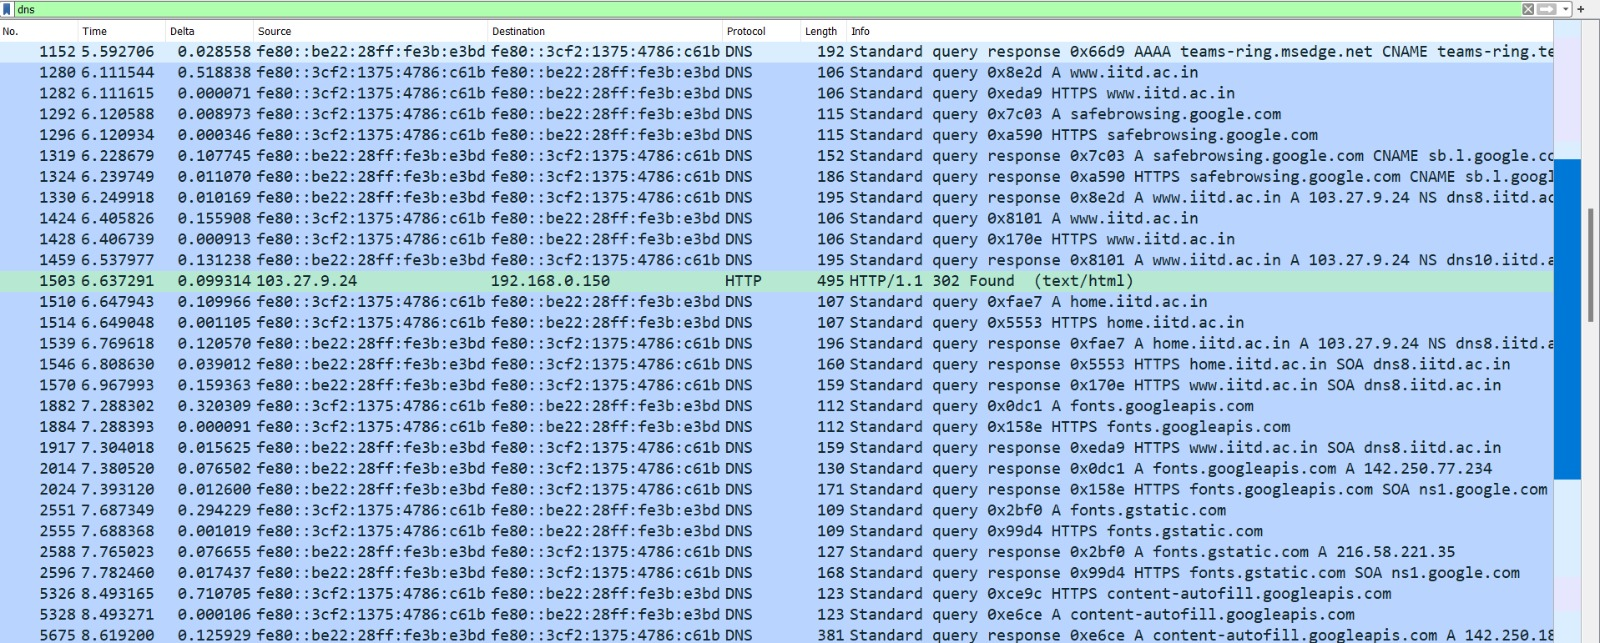
\includegraphics[width=15cm, height=6cm]
        {iitd-dns.jpeg}
            \item The analysis of the captured packet trace using Wireshark revealed a time difference of 30.6 milliseconds between the initiation of the DNS request and the receipt of the corresponding DNS response.
           \end{itemize}
        \item \textbf{For http://act4d.iitd.ac.in}
        \begin{itemize}
            \item 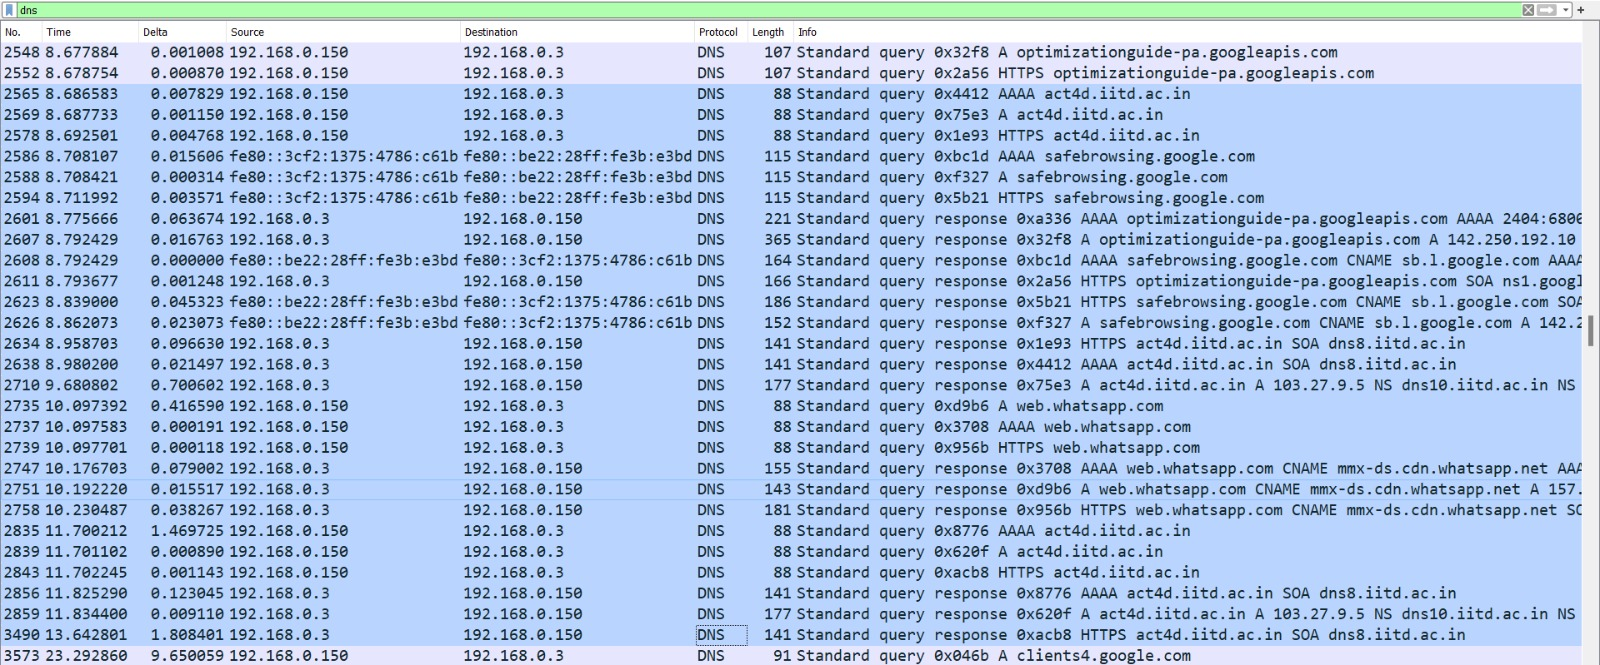
\includegraphics[width=15cm, height=7cm]
            {act4d-dns.jpeg}
            \item The analysis for this website using Wireshark revealed a time difference of approximately 5 milliseconds between the initiation of the DNS request and the receipt of the corresponding DNS response.
        \end{itemize}
        \end{itemize}
    \item b) \textbf{HTTP Requests in Packet Trace}:
        \begin{itemize}
            \item \textbf{For www.iitd.ac.in}
            \begin{itemize}
            % \item \includegraphics[width=15cm, height=2cm]
            % {priya-c.jpeg}
            % \item The HTTP requests in the above screenshot were the ones that were frequently identified
            % \item Upon applying the "HTTP" filter to the packet trace in Wireshark, it was observed that six HTTP-related entries were captured.
            % \item The GET request represents the initial request made by the browser to retrieve the main HTML  content of the webpage.
            % \item The HTTP response with the status code "302 Found" indicates a redirection. It suggests that the resource has temporarily moved to a different location and the browser is instructed to fetch the content from another URL.
            % \item The next response indicates a POST request that might be related to fetching additional resources or information required to render the webpage.
            % \item The response with the status code "302 Modified Temporarily" suggests a temporary modification of the requested resource.
            % \item The last response indicates a successful communication between the browser and the server. The "200 OK" status code confirms that the server has successfully processed the request and sent the requested resources to the browser.
            % \item The subsequent triggers for additional resources like images, stylesheets, scripts and other assets, initiate only after the initial HTML request. Web browsers initially process the provided HTML content, and subsequently, they pursue included links and references to retrieve extra resources(images, CSS, JavaScript). This collective effort leads to the comprehensive display of a webpage.
            \item 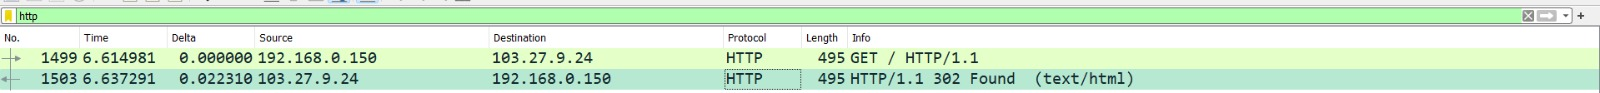
\includegraphics[width=15cm, height=1cm]
            {iitd-http.jpeg}
            \item We can see that there is only one unique HTTP request identified.
            \item This underlines the security controls put in place by the website to protect the privacy and accuracy of data transmission.
            \end{itemize}
        \item \textbf{For http://act4d.iitd.ac.in}
        \begin{itemize}
            \item 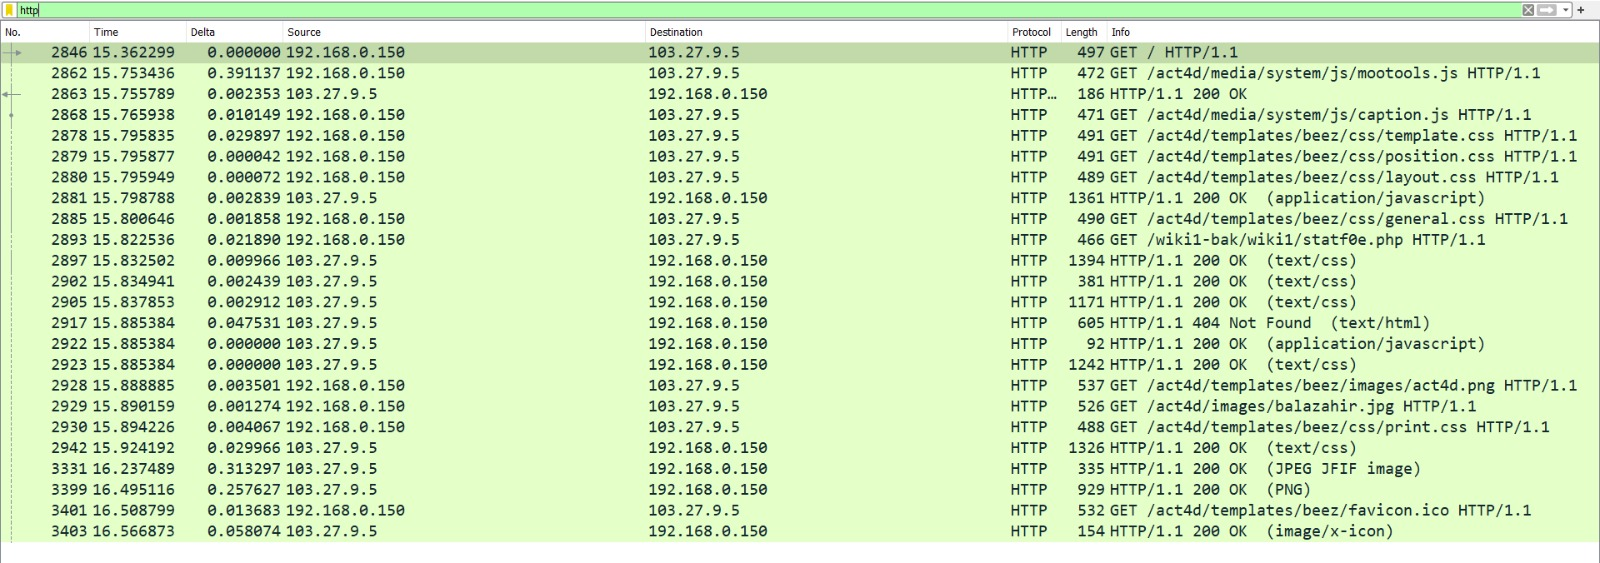
\includegraphics[width=15cm, height=6cm]
            {act4d-http.jpeg}
            \item A total of \textbf{12} distinct HTTP requests were generated and their corresponding 12 responses were generated.
            \item The provided screenshot shows that the browsing experience follows a recognizable pattern. The client starts the communication by asking for the basic HTML, then particular JavaScript files like "mototools.js" and "caption.js." The process then moves on to fetching several CSS files like "template.css," "position.css," "layout.css," and "general.css." 
            \item GET request for image and files in HTTP and response to it helps the browser to render complex images and files. If the HTML response contains references to external resources like images, CSS files, or scripts, the browser fetches these resources using separate HTTP requests.
        \end{itemize}
        \item Websites are structured using HTML, CSS and JavaScript. The browser first parses the HTML content, after which there are subsequent triggers resources like images, stylesheets, scripts and other assets. This collective effort leads to the comprehensive display of a webpage.
        \end{itemize}
        
    \item c) \textbf{Investigating TCP Connections} 
     \begin{itemize}
         \item \textbf{For www.iitd.ac.in}:
            \begin{itemize}
            \item A total of \textbf{10} distinct TCP connections were identified between the browser and the web server.
            \item We identified only one unique HTTP request as the website is highly encrypted.
        \end{itemize}
        \item \textbf{For http://act4d.iitd.ac.in}:
        \begin{itemize}
            \item A total of \textbf{6} distinct TCP connections were identified between the browser and the web server.
            \item The number of HTTP requests is \textbf{12} which is greater than the number of TCP connections. 
        \end{itemize}
        \item Upon applying the network filter, it was observed that several TCP connections were established between the browser and the web server.
        \item Comparing the number of TCP connections with the number of HTTP requests, the number of HTTP requests was more than the number of TCP requests. This is because a single TCP connection was used to fetch multiple HTTP requests. This enhances efficiency by minimising the need to create new connections for every resource.
        \item Furthermore, it was observed that some content objects were indeed fetched over the same TCP connection. For example, we noticed that some CSS files and images were fetched over a same TCP connection.
     \end{itemize}
    \item d) On doing the HTTP filter in Wireshark, there was no or very less HTTP traffic coming from www.indianexpress.com. The reason for this could be that HTTP traffic is encrypted, so Wireshark won't be able to decipher the payload of the packets unless we have administrative rights or an SSL encryption key. We won't be able to see the content of HTML and javascript files being transferred as explained above, the content of the packets will be encrypted and we constantly get encryption alerts in the trace. This is a security feature that ensures data privacy during transmission. \\
    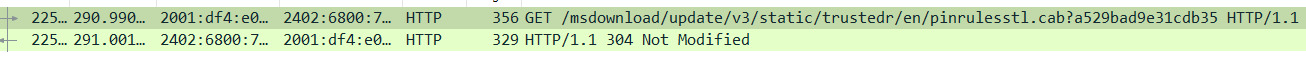
\includegraphics[width=15cm, height=1cm]{http-for-indian-express.jpeg}
\end{itemize}
\end{document}

